%\chapter{Schrotrauschen}

%\FloatBarrier
%\begin{figure}[htbp]
%    \centering
%    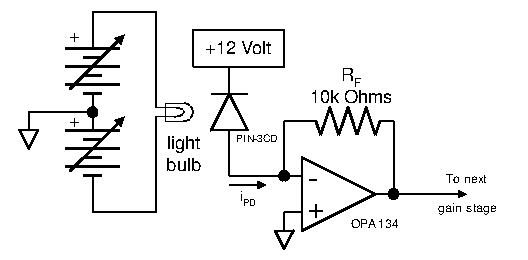
\includegraphics[width=0.5\textwidth]{figs/schrot schaltung.png}
%    \caption{Schaltung fur die LLE-Box zur Beobachtung des Schrotrauschens \cite{praktikum}}
%    \label{fig:schrotschaltung }
%\end{figure}
%\FloatBarrier

%\FloatBarrier
%\begin{figure}[htbp]
%    \centering
%    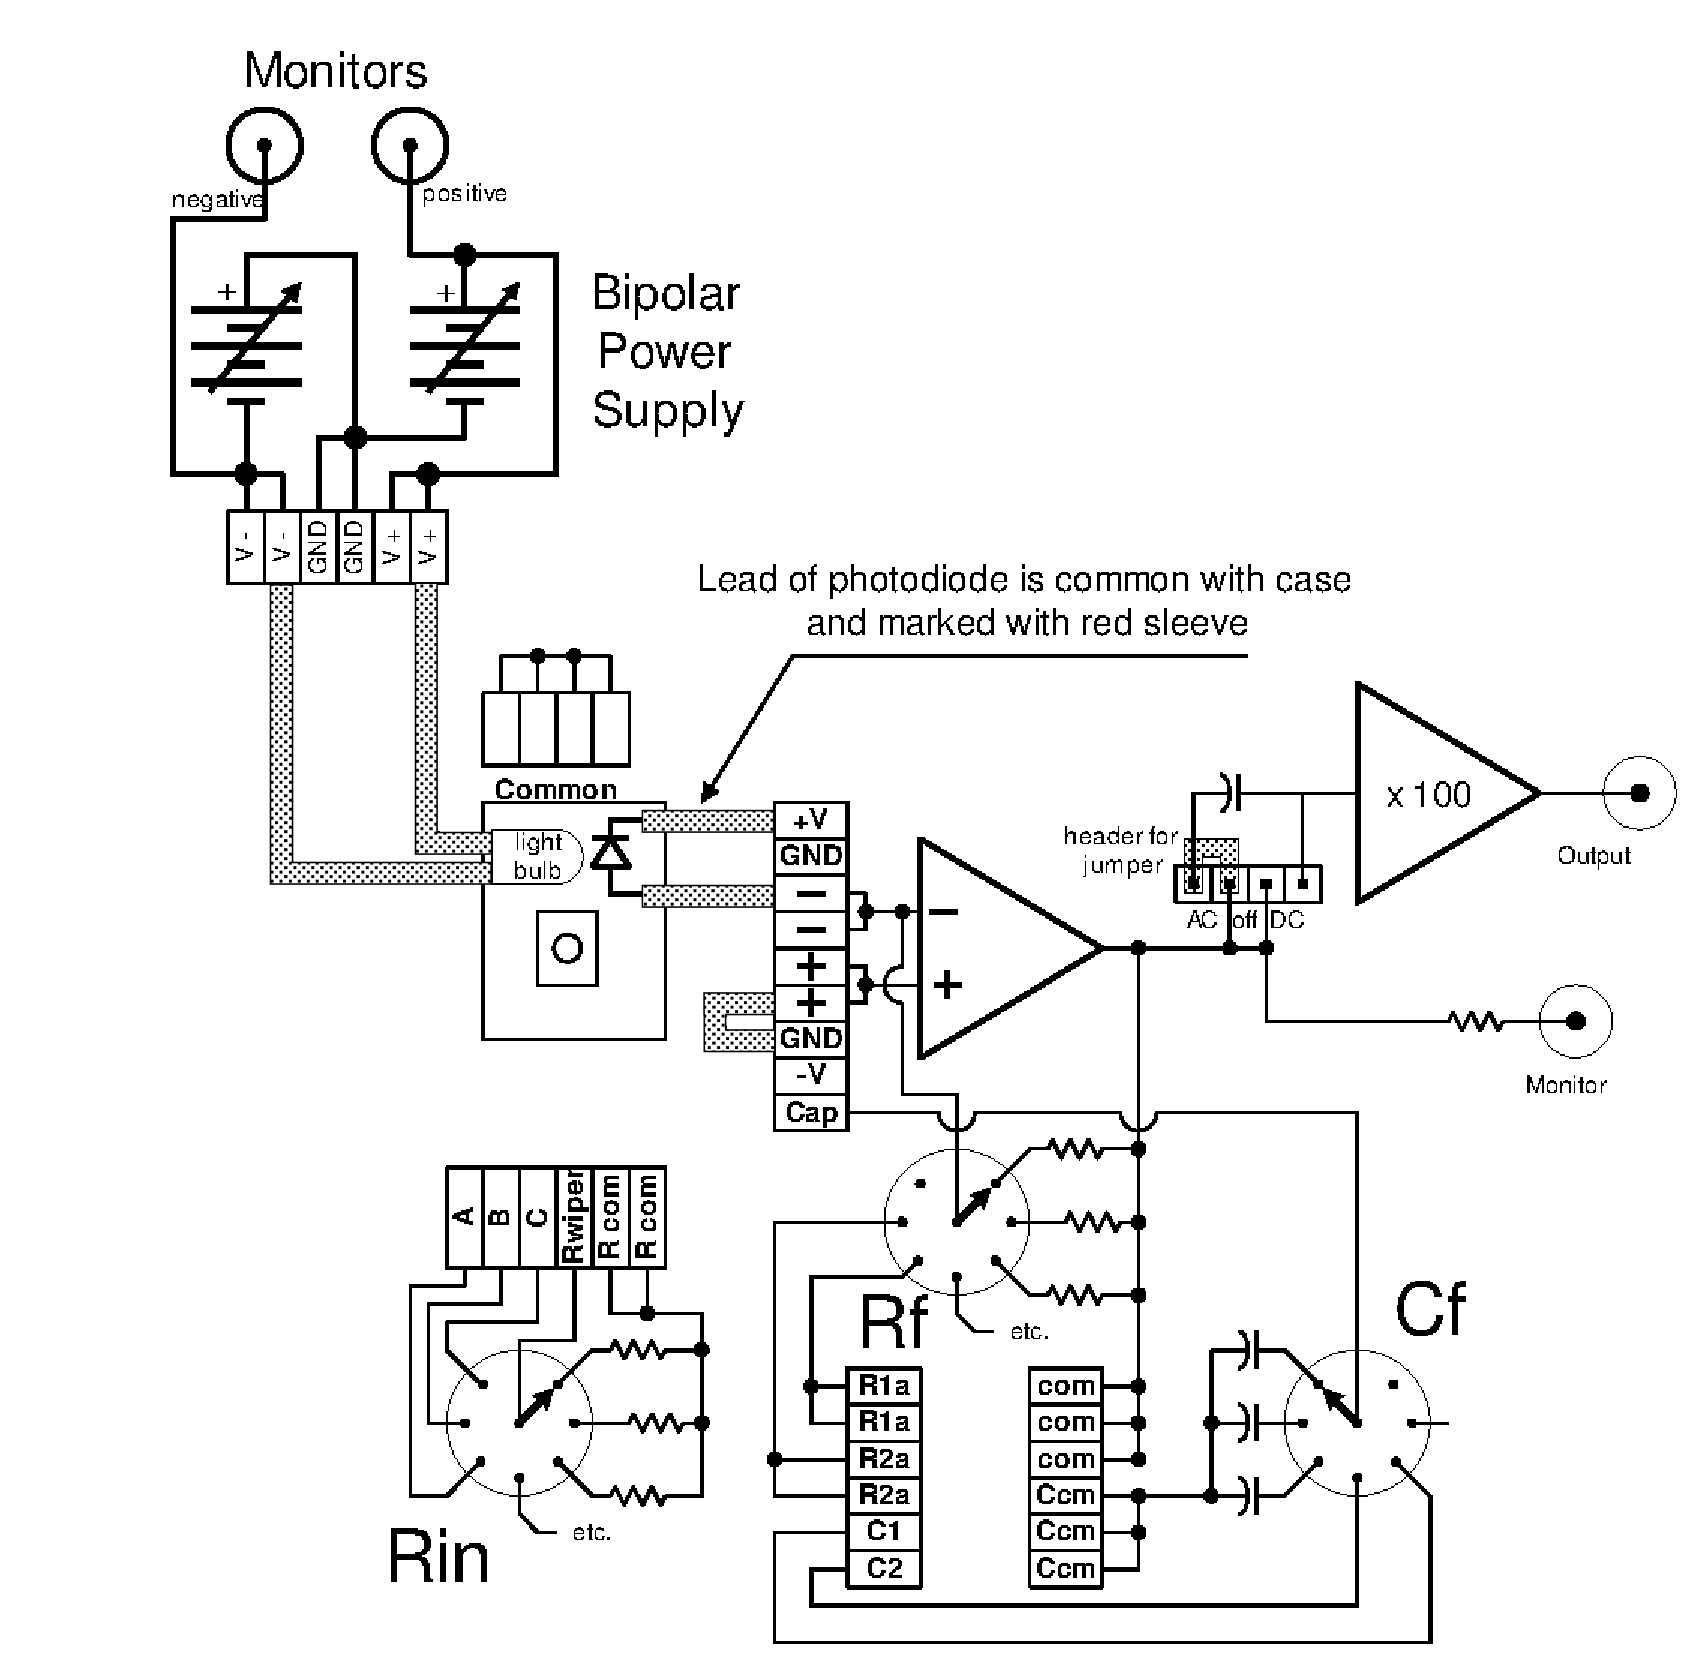
\includegraphics[width=0.5\textwidth]{figs/schrot lle.png}
%    \caption{Interner Schaltplan der LLE-Box zur Beobachtung des Schrotrauschens \cite{praktikum}}
%    \label{fig:schrotlle}
%\end{figure}
%\FloatBarrier

%\section{Beobachten des Schrotrauschens}
%\FloatBarrier
%\begin{figure}[htbp]
%    \centering 
%    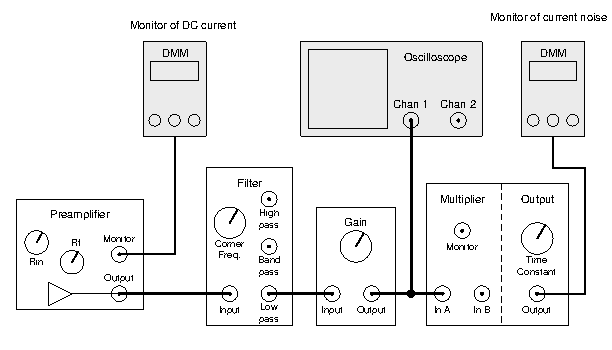
\includegraphics[width=0.5\textwidth]{figs/schrot hle.png}
%  \caption{Schaltung der HLE-Box zur Beobachtung des Schrotrauschens \cite{praktikum}}
 %   \label{fig:schrothle}
%\end{figure}
%\FloatBarrier

%

